\chapter{Evaluation and Future Work}
\section{Evaluating Performance}

In order to test the Block Explorer's performance, time measurements were taken for certain actions. 
The first measurement that was taken, measured the time it took to retrieve all blockchain data, process it and store it in the SQL database. The blockchain that was used for this test consisted of over fifteen thousand blocks. It is important to note, that the majority of the blocks were empty, meaning no transactions were included in them. The miner, the explorer connects to, was hosted on an Ubuntu \cite{ubuntu} Virtual Machine, located at the University of Zurich. In Table \ref{tab:load}, the average load times on different machines with varying hard and software are presented. 

It is noticeable that, by increasing CPU power and available RAM, the average load time reduces significantly. By design, the explorer retrieves the most recent data first. The explorer can access the already processed data and present it to a user, while more data is being loaded during the explorer's start up. This means that long initial load times to fill the database, due to slow hardware, are not an issue that directly affect a user's experience. Especially since most users are interested in the most recent data, for example when they wish to check on their latest transactions.

Another measurement that was taken, consisted of the time it took to request and display single items, lists of items and the search function. The results are displayed in Table \ref{tab:query}. In this test, the explorer itself was hosted on an Ubuntu Virtual Machine at the University of Zurich and already processed the blockchain with over fifteen thousand blocks. The \emph{HTML Load Time} column in Table \ref{tab:query} measured the time it took from the request to the server, until it responded with the HTML file containing the requested blockchain data. Since other files are being loaded, such as style sheets, the time to load the entire page is included in the table as well. Testing was conducted using a Computer, connected the University's Network using ethernet and timed using Google Chrome's \cite{chrome} developer tools.
\newpage
Comparing the results of the load times of Table \ref{tab:query} to similar requests made on Blockexplorer.com \cite{blockexplorer} and Etherscan.io \cite{etherscan}, the Bazo Block Explorer provided faster responses than the existing block explorers. This makes inspecting blockchain data on the Bazo Blockchain Explorer a satisfactory experience. Even when using a VPN to simulate long network distances, the load times were slightly lower on the Bazo Blockchain Explorer. It has to be noted, that Bitcoin and Ethereum blockchain sizes are far larger than the used Bazo dataset \cite{bitinfo} and the processing power of the existing explorer's servers is unknown.

\begin{table}[]
\centering
\caption{Load Times to Copy Fifteen Thousand Blocks From a Miner}
\label{tab:load}
\begin{tabular}{|l|l|l|l|}
\hline
\textbf{Computer} & \textbf{CPU} & \textbf{RAM} & \textbf{Load Time in Minutes} \\ \hline
MacBook Pro & 2.9 GHz Intel Core i5 & 8 GB & 2:17 \\ \hline
Ubuntu VM & 2.4 GHz  Intel Xeon & 2 GB  & 3:29 \\ \hline
\end{tabular}
\end{table}

\begin{table}[]
\centering
\caption{Load Times for Various Requests}
\label{tab:query}
\begin{tabular}{|l|l|l|}
\hline
\textbf{Query}            & \textbf{HTML Load Time} & \textbf{Page Load Time} \\ \hline
Block                     & 25 ms                   & 122 ms                  \\ \hline
Funds Transaction         & 30 ms                   & 121 ms                  \\ \hline
Account with Transactions & 32 ms                   & 119 ms                  \\ \hline
100 Most Recent Blocks    & 63 ms                   & 152 ms                  \\ \hline
Status Page               & 70 ms                   & 744 ms                  \\ \hline
Search of a Block         & 62 ms                   & 151 ms                  \\ \hline
\end{tabular}
\end{table}

\section{Future Work}
At time of writing, the applications's backend functionality of retrieving blocks from a miner, saving them to the database and returning them upon request is separated from the frontend that displays the returned data. This enables the possibility of switching out the frontend that displays HTML content for a REST API that returns the blockchain data in JSON format. Uses of such an interface could be an integration into the Payment System PWA, which displays data only on request. For example the PWA could display all confirmed transactions for an account in order to make the Payment app more informative, as seen in Figure \ref{fig:pwa_api}.

Another feature, the current block explorer lacks, is frontend optimization for mobile devices. Dynamically styled tables and UI components are needed to accommodate for the many resolutions and aspect ratios of mobile devices. To increase performance, especially on mobile devices, CSS micro-frameworks, such as Furtive \cite{furtive} or Pure.CSS \cite{pure} could be used to keep style sheets at a minimum size. This would also prevent the need for resource-heavy Bootstrap imports and links.
\\
\\
\\

\begin{figure}[h]
  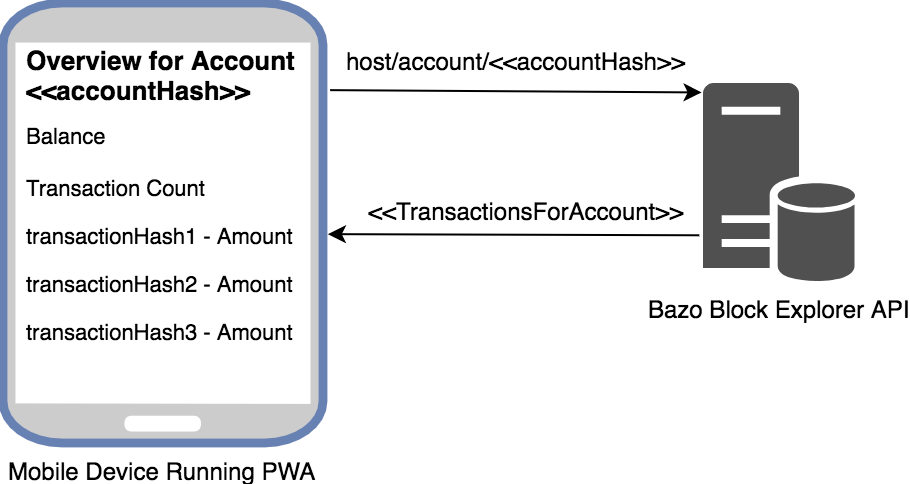
\includegraphics[scale=0.4]{pwa_integration.png}
  \centering
  \caption{Device Running PWA Payment System Requesting a User's Transactions}
  \label{fig:pwa_api}
\end{figure}